\section{Classical Mechanics}

The following subsections cover the basic knowledge needed for the classical mechanics questions on the exam.
The first subsection simply provides a quick reference for essential equations.
However, simply stating conservation of momentum is no substitute for actually working out several problems using conservation of momentum.
As such, the fist section is deceptively concise.
Most of the time studying this section should be spent brushing up on skills to use equations from the Basic Mechanics subsection.
The second subsection is over Lagrangian and Hamiltonian mechanics and reviews the basic equations involved.
There is no substitute for constructing the kinetic energy and potential energy in terms of generalized coordinates for yourself.
The subsequent subsections go into more detail about topics such as gravitation, normal modes, and mechanical waves.
An excellent quantitative and qualitative understanding of this section is necessary for the PGRE.

\subsection{Basic Mechanics}

\subsubsection{Translational and Rotational Kinematics}

The following are derived from:\\
\( \mathbf{a} = \mathrm{const.} \),  \(a = \frac{\mathrm{d}v}{\mathrm{d}t} =  v\frac{\mathrm{d}v}{\mathrm{d}x}  \),  \( v=\frac{\mathrm{d}x}{\mathrm{d}t} \)\\
\(  \vec{\alpha} = \mathrm{const.} \),  \(\alpha = \frac{\mathrm{d}\omega}{\mathrm{d}t} =  \omega\frac{\mathrm{d}\omega}{\mathrm{d}\theta}  \),  \( \omega=\frac{\mathrm{d}\theta}{\mathrm{d}t} \)
\begin{itemize}
\item \( \Delta s = v_0 t + \frac{1}{2} a t^{2} \)
\item \( \Delta v = a t \)
\item \( v^2 -  v_0^2 =  2a \Delta s \)
\item \( \Delta \theta = \omega_0 t + \frac{1}{2} \alpha t^{2} \)
\item \( \Delta \omega = \alpha t \)
\item \(  \omega^2 -   \omega_0^2 =  2\alpha \Delta \theta \)
\end{itemize}
Projectile motion:\\* \( y_{max}=\frac{v_0^2 \sin^2(\theta)}{2g} \)\\* \( x_{max}=\frac{v_0^2 \sin(2\theta)}{g} \)\\\\*
Circular motion:\\* \(s_{arc}=R\theta\)\\* \( v_{tangential}=R\omega \)\\* \(a_{centripetal}=\frac{v_{tangential}^2}{R}=R\omega^2\)\\* \( a_{tangential}=R\alpha \)

\subsubsection{Rotations}
Moment of Inertial (for symmetric bodies): \(I=\sum_im_i(r_{\bot})_i^2 \to \int r_{\bot}^2\,dm\)\\*
(\(r_{\bot}\) is the perpendicular distance from the axis of rotation)
\newpage
Common moments of inertial:
\begin{center}
 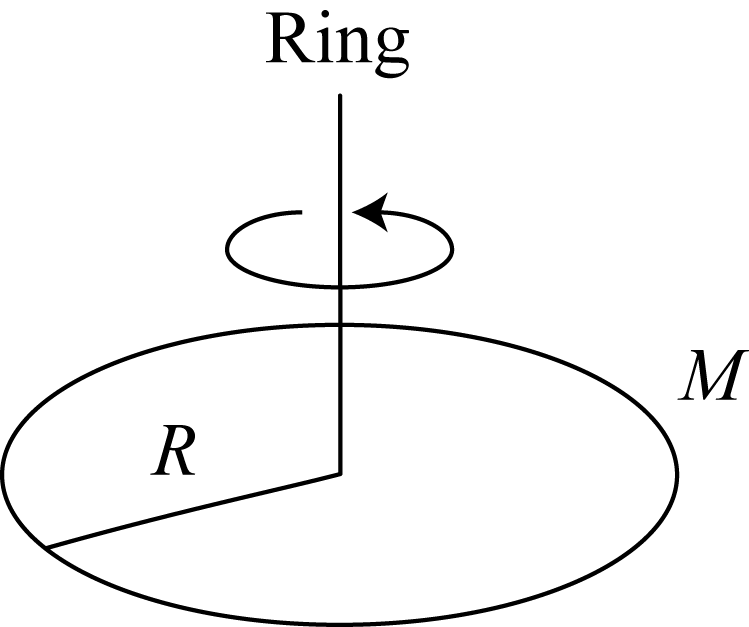
\includegraphics[scale=0.5]{images/PGRE_Figures_1p1p2_Ring.png}
 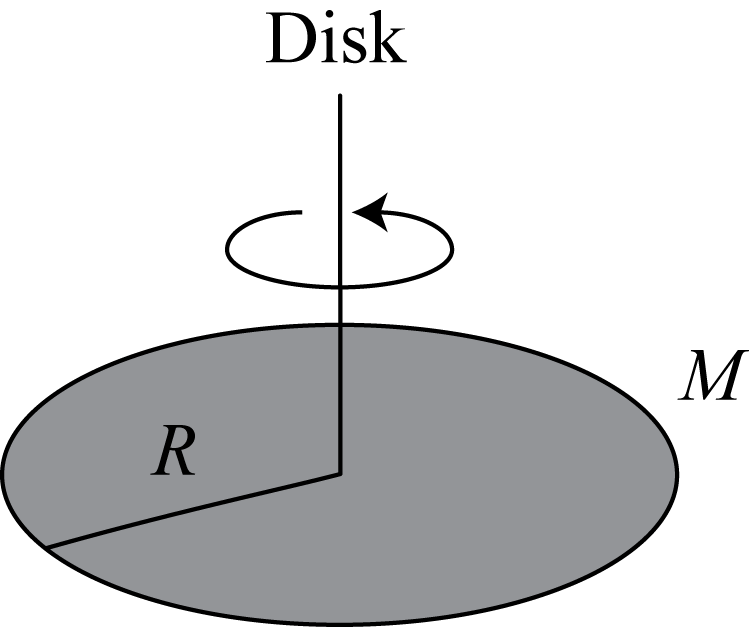
\includegraphics[scale=0.5]{images/PGRE_Figures_1p1p2_Disk.png}
 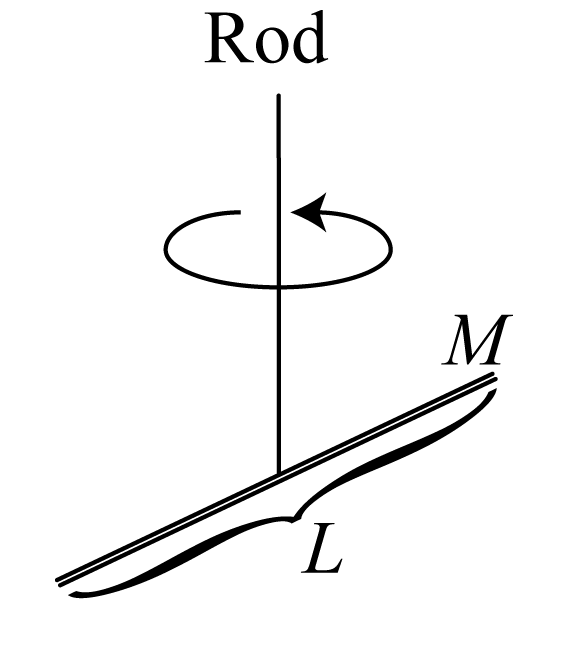
\includegraphics[scale=0.5]{images/PGRE_Figures_1p1p2_Rod.png}
 \end{center}
\begin{itemize}
\item Ring: \(I=MR^2\)
\item Disk: \(I=\frac{1}{2}MR^2\)
\item Rod: \(I=\frac{1}{12}ML^2\)
\item Solid Sphere: \(I=\frac{2}{5}MR^2\)
\item Spherical Shell: \(I=\frac{2}{3}MR^2\)
\end{itemize}
Know which dimensions are important for calculating moments of intertial.
(e.g.: A cylinder of length \(L\) that rotates about its length has the same moment of inertial as a disk rotating about the same axis.)\\*
Derivation of \(I\) for a solid sphere: \\*
(Slice sphere into thin disks of radius \(R_{\bot}\) and thickness \(\mathrm{d}z\))
\begin{eqnarray}
\mathrm{d}I_{disk}&=&\frac{1}{2}R_{\bot}^2\mathrm{d}m \nonumber \\
\mathrm{d}m &=& \rho\pi R_{\bot}^2\mathrm{d}z \nonumber \\
I_{sphere}=\int_{-R}^{R}\frac{1}{2}\pi\rho R_{\bot}^4\mathrm{d}z &=& \int_{-R}^{R}\frac{1}{2}\pi\rho (R^2-z^2)^2\mathrm{d}z \nonumber \\
I_{sphere}=\frac{8}{15}\pi\rho R^5 &=& \frac{2}{5}MR^2 \nonumber
\end{eqnarray}
Parallel axis theorem: \(I=I_{CM}+Md^2\)\\*
Radius of Gyration: \(R_{gyration}=\sqrt{I/M}\)\\\\*
Review rolling without slipping.\\\\*
Torque: \(\vec{\tau}=\mathbf{r}\times\mathbf{F}\)\\*
Angular Momentum: \(\mathbf{L}=\mathbf{r}\times\mathbf{p}=I\vec{\omega}\)

\subsubsection{Momenta}
\(\mathbf{p}=m\mathbf{v}\)\\*
\(\mathbf{L}=\mathbf{r}\times\mathbf{p}\)\\\\*
Both \( \mathbf{p} \) and \( \mathbf{L} \) are conserved if there are no external forces acting on the bodies.\\*
\(\Delta \mathbf{p}=\mathbf{p}_f-\mathbf{p}_i=0\)\\*
\(\Delta \mathbf{L}=\mathbf{L}_f-\mathbf{L}_i=0\)

\subsubsection{Newton's Second Law}
\( \displaystyle\sum_{i}\mathbf{F_{\mathit{i}}}=\frac{\mathrm{d}\mathbf{p}}{\mathrm{d}t} \) \(\to\) \( \displaystyle\sum_{i}\mathbf{F_{\mathit{i}}}=m\mathbf{a} \) when \(\mathit{m} = \mathrm{const.}\)\\*
\( \displaystyle\sum_{i}\vec{\tau}_{\mathit{i}}=\frac{\mathrm{d}\mathbf{L}}{\mathrm{d}t} \) \(\to\) \( \displaystyle\sum_{i}\vec{\tau}_{\mathit{i}}=I\vec{\alpha} \) when \(I = \mathrm{const.}\)\\\\*
Statics:\\*
\( \displaystyle\sum_{i}\mathbf{F_{\mathit{i}}}=m\mathbf{a} =\vec{0}\)\\*
\( \displaystyle\sum_{i}\vec{\tau}_{\mathit{i}}=I\vec{\alpha} =\vec{0}\)\\\\*
Frictional force:\\*
\( F_{fric}=\mu N \)  where \(N\) is the normal force on the object\\\\*
Pulleys:
\begin{center}
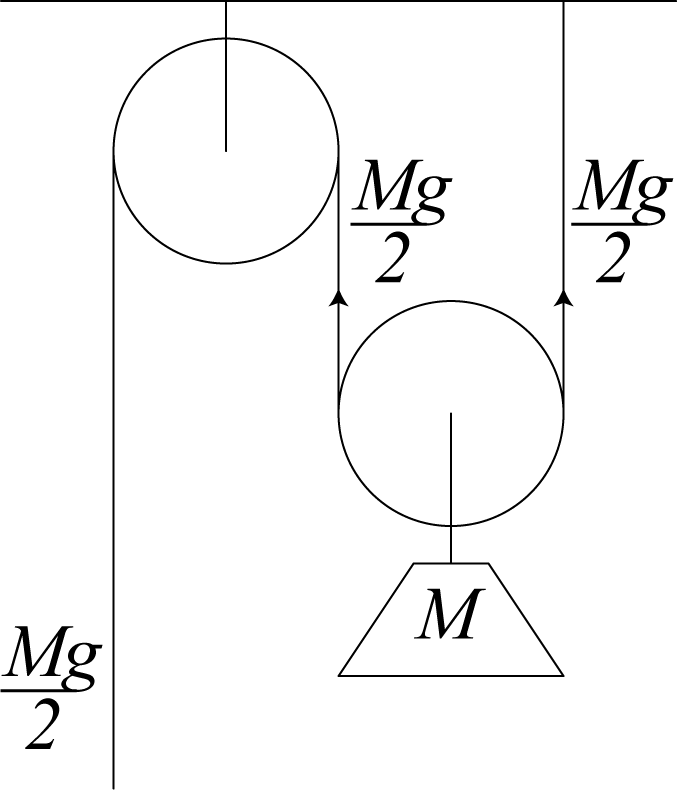
\includegraphics[scale=0.5]{images/PGRE_Figures_1p1p4_Pulleys.png}
\end{center}
\begin{enumerate}
\item Tension is uniform throughout the rope.
\item When the rope is anchored to a support the pulley system acts as a force multiplier.
\end{enumerate}

\subsubsection{Fictitious Forces}
\(\mathbf{F}'=\mathbf{F}_{physical}-m\mathbf{A}_0-2m\vec{\omega}\times \mathbf{v}'-m\dot{\vec{\omega}}\times \mathbf{r}'-m\vec{\omega}\times\left( \vec{\omega}\times\mathbf{r}' \right)\)\\\\*
\(\mathbf{F}_{physical}\) are any true forces from an inertial perspective\\*
\(\mathbf{A}_0\) is the acceleration of the entire frame\\*
\(\mathbf{F}_{Coriolis}=-2m\vec{\omega}\times \mathbf{v}'\)\\*
\(\mathbf{F}_{transverse}=-m\dot{\vec{\omega}}\times \mathbf{r}'\)\\*
\(\mathbf{F}_{centrifugal}=-m\vec{\omega}\times\left( \vec{\omega}\times\mathbf{r}' \right)\)\\\\*
At Earth's surface:\\*
\(\mathbf{F}_{transverse}=\mathbf{0}\)\\*
\(\mathbf{F}_{centrifugal}\approx\mathbf{0}\)\\*
\(m\mathbf{g}_0-m\mathbf{A}_0=m\mathbf{g}\)\\\\*
Therefore, \(\mathbf{F}'=\mathbf{F}_{physical}+m\mathbf{g}-2m\vec{\omega}\times \mathbf{v}'\)\\\\*
If one defines a coordinate system where \(\hat{x}'\) is "east," \(\hat{y}'\) is "north," and \(\hat{z}'\) is "vertical," then \(\vec{\omega}=\omega\cos{\lambda}\hat{y}'+\omega\sin{\lambda}\hat{z}'\) (where \(\lambda\) is the latitude)

\subsubsection{Work and Energy}
Work-Kinetic Energy Theorem:\\*
\(\displaystyle W_{trans}=\int \mathbf{F}\cdot\,\mathrm{d}\mathbf{s}=\Delta K_{trans}\)\\*
\(\displaystyle W_{rot}=\int \tau\,\mathrm{d}\theta=\Delta K_{rot}\)\\*
\(K_{trans}=\frac{1}{2}mv^2\)\\*
\(K_{rot}=\frac{1}{2}I\omega^2\)\\\\*
Potential Energies:\\*
\(U_{gravity}=mgh\)\\*
\(U_{spring}=\frac{1}{2}kx^2\)\\
In general (for a conservative force \(\nabla\times\mathbf{F}=0\)): \(\mathbf{F}=-\nabla\cdot U\)\\\\*
Conservation of energy can only be used in special circumstances:\\*
\(\Delta E=E_f-E_i=K_f+U_f-(K_i+U_i)=0\)\\\\*
Energy Dissipated Through a Frictional Force: \(E_{lost}=\mu F_Nd\)

\subsubsection{Power and Impulse}
Power:\\*
\(P=\frac{\mathrm{d}W}{\mathrm{d}t} \)\\*
\( P=\mathbf{F}\cdot\mathbf{v}\) when \( \mathbf{F}=\mathrm{const.} \)\\*
\( P=\tau\omega\) when \( \vec{\tau}=\mathrm{const.} \)\\\\*
Impulse:\\*
\(I=\Delta p=\int F\,\mathrm{d}t\)\\*
\(H=\Delta L=\int \tau\,\mathrm{d}t\)

\subsubsection{Collisions}
In general, use conservation and momentum and energy for non-relativistic collisions.\\*
\(\Delta \mathbf{p}=0\) for both elastic and inelastic collisions\\*
\(\Delta \mathbf{L}=0\) for both elastic and inelastic collisions\\*
\(\Delta E=0\) only for elastic collisions\\\\*
Linear Elastic Collisions (no rotation or interaction potential):\\*
Factoring the kinetic energy and dividing by the momentum yields these two equations\\*
\( v_{1i} + v_{1f} = v_{2i} + v_{2f} \)\\*
\(m_1 v_{1i}+m_2v_{2i}=m_1 v_{1f}+m_2v_{2f}\)

\subsubsection{Many Particle Systems}
Center of Mass for Discrete Particles: \(\displaystyle \mathbf{r}_{CM}=\frac{\sum_{i} m_i\mathbf{r}_i}{\sum_{i} m_i}=\frac{\sum_{i} m_i\mathbf{r}_i}{M}\)\\*
Components:\\*
\(x_{CM}=\frac{\sum_{i} m_i x_i}{M}\)\\*
\(y_{CM}=\frac{\sum_{i} m_i y_i}{M}\)\\*
\(z_{CM}=\frac{\sum_{i} m_i z_i}{M}\)\\\\*
 Center of Mass for a Continuous Mass Distribution:\\*
 \(x_{CM}=\frac{\int_{V} \rho x\mathrm{d}V}{M}\)\\*
 \(y_{CM}=\frac{\int_{V} \rho y\mathrm{d}V}{M}\)\\*
 \(z_{CM}=\frac{\int_{V} \rho z\mathrm{d}V}{M}\)\\\\*
 Total momentum: \(\mathbf{p}_{CM}=M\mathbf{v}_{CM}\)\\*
 Total angular momentum: \(\displaystyle\mathbf{L}=\mathbf{r}_{CM}\times M\mathbf{v}_{CM} + \sum_{i}\bar{\mathbf{r}}_i \times M\bar{\mathbf{v}}_i\)\\*
 where \(\bar{\mathbf{r}}_i = \mathbf{r}_i-\mathbf{r}_{CM}\) and \(\bar{\mathbf{v}}_i = \mathbf{v}_i-\mathbf{v}_{CM}\)\\\\*
 The Rocket Equation: \(m\dot{\mathbf{v}}=\mathbf{F}_{ext}+\dot{m}\mathbf{v}_{rel}\)\\*
 \(\mathbf{v}_{rel}\) is the velocity of the propellent\\*
 (Note that this is NOT derived from Newton's second law! It's derived from impulse considerations.)

\subsubsection{Fluid Mechanics}
Pressure (force/area):\\*
\(P=\frac{F}{A}\)\\*
Conservation of mass (for incompressible, irrotational fluids) yields\\*
\(A_1v_1=A_2v_2\) where \(A\) is the cross sectional area and \(v\) is the speed of the fluid\\*
Conservation of energy yields (Bernoulli's equation)\\*
\(P_i+\rho_igh_i+\frac{1}{2}\rho_iv_i^2=\mathrm{const.}\) where \(\rho\) is the density of the fluid\\\\*
Review capillary action.

\subsection{Lagrangian \& Hamiltonian Mechanics}
%For this subsection \(K\to T\) and \(U\to V\).

\subsubsection{Lagrangian Mechanics}
The Lagrangian: \(L=L(q_1,\ldots,q_n,\dot{q}_1,\ldots,\dot{q}_n,t)=T-V\)\\*
(Kinetic energy minus the potential energy)\\*
Review generalized coordinates to see how to construct \(T\) and \(V\).\\*
Lagrange's equation: \(\displaystyle\frac{\partial L}{\partial q}=\frac{\mathrm{d}}{\mathrm{d}t}\left(\frac{\partial L}{\partial \dot{q}}\right)\)\\\\*
Lagrange's equation is derived from finding the extremum of the action integral \(\displaystyle S=\int_{t_1}^{t_2}L\,\mathrm{d}t\)

\subsubsection{Forces of Constraint}
Consider a system with \(n\) generalized coordinates and \(m\) equations of constraint \(f_j\)
\begin{eqnarray}
i&=&1,2,\ldots,n \nonumber \\
j&=&1,2,\ldots,m \nonumber \\
f_j(q_i,t) &=& 0 \nonumber \\
\frac{\mathrm{d}}{\mathrm{d}t}\frac{\partial L}{\partial \dot{q}_i}&=&\frac{\partial L}{\partial q_i}+\sum_j\lambda_j(t)\frac{\partial f_j}{\partial q_i} \nonumber
\end{eqnarray}
\(\sum_j\lambda_j(t)\frac{\partial f_j}{\partial q_i}\) is referred to as the force of constraint.

\subsubsection{Hamiltonian Mechanics}
The Hamitonian: \(H=H(q_1,\ldots,q_n,p_1,\ldots,p_n,t)= \sum_{i=1}^{n} p_i\dot{q}_i-L=T+V\)\\*
Hamilton's equations:
\begin{itemize}
\item \(\displaystyle\dot{q}=\frac{\partial H}{\partial p}\)
\item \(\displaystyle\dot{p}=-\frac{\partial H}{\partial q}=\frac{\partial L}{\partial q}\)
\item \(\displaystyle\frac{\partial H}{\partial t}=-\frac{\partial L}{\partial t}\)
\end{itemize}
Another useful relation is \(p=\frac{\partial L}{\partial \dot{q}}\)\\\\*
If \(t\) doesn't explicitly appear in the Lagrangian, then it will not be in the Hamiltonian and the Hamiltonian will be a constant of motion (conservation of energy).\\*
An ignorable (or cyclical) coordinate is one in which does not appear explicitly in the Lagrangian. (e.g. If \(q_n\) is an ignorable coordinate, then \(L=L(q_1,\ldots,q_{n-1},\dot{q}_1,\ldots,\dot{q}_n,t)\))

\subsection{Gravitation}
Newton's law of universal gravitation:\\*
\(\displaystyle\mathbf{F}_{gravity}=-G\frac{m_1m_2}{r_{12}^2}\hat{r}_{12}\)\\*
For an object near the surface of the earth:\\*
\(\mathbf{F}_{gravity}=-mg\hat{e}_r\)

\subsubsection{Kepler's Laws}
\begin{enumerate}
\item All planets' orbits are elliptical in shape. This is due to the inverse square nature of the gravitational force.\\*
Orbits are defined by their eccentricity:
\begin{itemize}
\item \(1<\epsilon\): hyperbolic orbit \(\to\) highest total orbital energy
\item \(\epsilon =1\): circular orbit \(\to\) any perturbation in orbital energy destroys this perfect orbit
\item  \(0<\epsilon < 1\): elliptical orbit \(\to\) most stable closed orbit
\item \(\epsilon = 0\): parabolic orbit \(\to\) has total orbital energy equal to zero
\end{itemize}
\item Each planet's orbit sweeps out an equal amount of area in an equal amount of time. This is due the conservation of angular momentum (\(L=mr^2\dot{\theta}=\mathrm{const.}\)).\\*
\(\frac{\mathrm{d}A}{\mathrm{d}t}=\frac{L}{2m}=\mathrm{const.}\)\\*
\(T_{period}=\frac{A_T}{\frac{\mathrm{d}A}{\mathrm{d}t}}=\frac{2mA_T}{L}\)
\item The square of the period of a planet is directly proportional to cube of its semi-major axis (\( T_{period}^2 \propto a^3\)). This law is easily derived for circular orbits (The law has the same form for elliptical orbits but that derivation is far beyond the scope of the PGRE).\\*
\begin{eqnarray}
\displaystyle\sum F_r=G\frac{Mm}{r^2}&=&ma_{centripetal}=mr\omega^2 \nonumber \\
G\frac{M}{r^3}&=&\left( \frac{2\pi}{T_{period}} \right)^2 \nonumber \\
T_{period}&=&\frac{2\pi}{\sqrt{GM}}r^{3/2}  \nonumber
\end{eqnarray}
In general: \(\displaystyle T_{period}^2=\frac{4\pi^2}{GM}a^{3}\)\\*
This same type of derivation is used to find the orbital speed: \(v=\sqrt{\frac{GM}{r}}\)\\*
Notice that the period and orbital speed are not related to the mass of the orbiting body.\\*
If \(T_{period}\) is given in years and \(a\) is in A.U., then \(T_{period}^2=a^3\)\\*
If one is given information about a planet and its satellite:\\* \(\displaystyle\frac{m_{planet}}{M_{sun}}=\frac{r_{sat}^3T_{planet}^2}{r_{planet}^3T_{sat}^2}\)
\end{enumerate}

\subsubsection{Central Forces and Reduced Mass}
The total energy of an orbit is given by: \(E_T=\frac{1}{2}m\dot{r}^2+U_{eff}\)\\*
\(U_{eff}\) is the effective potential energy of the orbiting body: \(U_{eff}=\frac{L^2}{2mr^2}-\frac{GMm}{r}\)\\*
Virial Theorem: \(\overline{K}=-\frac{1}{2}\overline{\sum_i \mathbf{F}_i\cdot \mathbf{r}_i}\)\\*
If the force is derived from a central potential \(U=br^n\): \(\overline{K}=\frac{n}{2}\overline{U}\)\\*
The total energy for a body in a closed orbit is: \(E_T=\frac{-GMm}{2a}\)\\*
The escape velocity of an object is the speed needed to completely escape the gravitational pull of a massive object.
It can be derived from considering the energy of a mass in a gravitational field:
\begin{eqnarray}
\Delta E&=&0 \nonumber \\
K_i+U_i&=&K_f+U_f\nonumber\\
\frac{1}{2}mv_i^2-\frac{GMm}{r}&=&0\nonumber\\
v_e&=&\sqrt{\frac{2GM}{r}}\nonumber
\end{eqnarray}
If one uses the surface of the Earth as the starting point: \(v_e=\sqrt{2gR_E}\)\\*
Bertrand's theorem: Only two types of potentials can produce stable, closed orbits; the inverse, central potential \(U(r)=\frac{-k}{r}\) and the radial harmonic oscillator \(U(r)=\frac{1}{2}kr^2\)\\\\*
The reduced mass of two bodies moving about their center of mass is \(\mu=\frac{m_1m_2}{m_1+m_2}\)\\*
Replace \(m\) in \(ma_{centripetal}\) with \(\mu\) to get Kepler's 3$^{\mathrm{rd}}$ law: \(T_{period}=\frac{2\pi}{\sqrt{G(m_1+m_2)}}a^{3/2}\)\\*
If \(a\) is in A.U. and \(T_{period}\) is in years, then \(T_{period}=\frac{1}{\sqrt{m_1+m_2}}a^{3/2}\)

\subsubsection{Orbital Equation}
\(l=\frac{L}{m}\) and \(u=\frac{1}{r}\) (where \(L\) is the angular momentum, not the Lagrangian)
\begin{itemize}
\item Conservation of Angular Momentum: \(r^2\dot{\theta}=l\)
\item Orbital Equation: \(\displaystyle\frac{\mathrm{d}^2u}{\mathrm{d}\theta^2}+u+\frac{1}{ml^2u^2}f(u^{-1})=0\)
\end{itemize}
Derivation of orbital equation(s) using Lagrange's equations:
\begin{eqnarray}
x&=&r\cos{\theta}  \nonumber \\
\dot{x}&=&\dot{r}\cos{\theta}-r\dot{\theta}\sin{\theta} \nonumber \\
y&=&r\sin{\theta} \nonumber \\
\dot{y}&=&\dot{r}\sin{\theta}+r\dot{\theta}\cos{\theta} \nonumber \\
T = \frac{1}{2}m(\dot{x}^2+\dot{y}^2) &=& \frac{1}{2}m(\dot{r}^2+r^2\dot{\theta}^2) \nonumber \\
L&=& \frac{1}{2}m(\dot{r}^2+r^2\dot{\theta}^2) - V(r) \nonumber
\end{eqnarray}
\(\theta\) is an ignorable coordinate
\begin{eqnarray}
\frac{\partial L}{\partial \theta}&=&0 \nonumber \\
\frac{\mathrm{d}}{\mathrm{d}t}\frac{\partial L}{\partial \dot{\theta}}&=&\frac{\mathrm{d}}{\mathrm{d}t}(mr^2\dot{\theta})  \nonumber
\end{eqnarray}
Hence, \(mr^2\dot{\theta} = const.\)\\*
Remember that \(f(r)=-\frac{\partial V}{\partial r}\)
\begin{eqnarray}
\frac{\partial L}{\partial r}&=&mr\dot{\theta}^2+f(r) \nonumber \\
\frac{\mathrm{d}}{\mathrm{d}t}\frac{\partial L}{\partial \dot{r}}&=&m\ddot{r}  \nonumber \\
m\ddot{r}&=&mr\dot{\theta}^2+f(r)  \nonumber \\
m\ddot{r}&=&m\frac{l^2}{r^3}+f(r)  \nonumber
\end{eqnarray}
Using \(\dot{r}=-l\frac{\mathrm{d}u}{\mathrm{d}\theta}\) and \(\ddot{r}=-u^2l^2\frac{\mathrm{d}^2u}{\mathrm{d}\theta^2}\)
\begin{eqnarray}
\frac{\mathrm{d}^2u}{\mathrm{d}\theta^2}&=&-u-\frac{1}{ml^2u^2}f(u^{-1}) \nonumber
\end{eqnarray}

\newpage

\subsection{Periodic Motion}
Angular frequency of small oscillations for various objects
\begin{itemize}
\item Physical pendulum: \(\omega_p=\sqrt{\frac{Mgd}{I}}\) where \(d\) is the distance from the support to the center of mass
\item Ideal pendulum (let \(d \to l\) and \(I \to Ml^2\)): \(\omega_p=\sqrt{\frac{g}{l}}\)
\item Mass on a spring: \(\omega_s=\sqrt{\frac{k}{m}}\)
\item In general: \(\omega=\sqrt{\frac{V_0''}{M}}\)\\*
\(V_0''\) is the second derivative of the potential energy evaluated at \(q=0\) (equilibrium).
\end{itemize}

\subsubsection{Simple Harmonic Motion}
Governing equation: \(\ddot{x}=-\omega_s^2x\)\\*
Solution: \(x(t)=A\sin(\omega_st-\phi)\)\\*
Total energy in a simple harmonic oscillator (SHO): \(E_T=\frac{1}{2}kA^2=\frac{1}{2}m\omega_s^2A^2\)\\*
Conservation of energy gives the speed of the mass \(v=\omega_s\sqrt{A^2-x^2}\)\\*
This only becomes obvious when studying capacitors: \(k_{parallel}=\sum_i k_i\) and \(\frac{1}{k_{series}}=\sum_i \frac{1}{k_i}\)\\*
Torsional pendulum: \(\tau=-\kappa\theta \to T_{period}=2\pi\sqrt{\frac{I}{\kappa}}\)

\subsubsection{Damped Harmonic Motion}
Governing equation: \(\ddot{x}=-2\gamma\dot{x}-\omega_s^2x\)\\*
Solution: \(x(t)=A_1e^{-(\gamma-q)t}+A_2e^{-(\gamma+q)t}\) where \(q=\sqrt{\gamma^2-\omega_s^2}\)\\*
The rate of energy loss in \emph{any} damped oscillator is \(\frac{\mathrm{d}E_T}{\mathrm{d}t}=-2m\gamma\dot{x}^2\)\\*
Total energy in a \emph{weakly} damped oscillator: \(E(t)=\frac{1}{2}m\omega_s^2A^2e^{-t/\tau}=E_0e^{-t/\tau}\)\\\\*
\(q\) determines how damped the system is
\begin{itemize}
\item \(0<q\): Overdamping \(\to\) ``oscillator'' will slowly return to equilibrium
\item \(q=0\): Critical damping \(\to\) \(x(t)=Ate^{-\gamma t}+Be^{-\gamma t}\)
\item \(q\in\Im\): Underdamping \(\to\) \(x(t)=Ae^{-\gamma t}\sin(\omega_dt+\phi)\) where \(\omega_d=\sqrt{\omega_s^2-\gamma^2}\)
\end{itemize}
The quality factor for a weakly damped oscillator is \(Q=\frac{\omega_d}{2\gamma}\)

\subsubsection{Forced Oscillation}
Governing equation: \(\ddot{x}=-2\gamma\dot{x}-\omega_s^2x+F_0\)\\*
Steady-state solution: \(\displaystyle A=\frac{F_0/m}{\sqrt{\left(\omega^2-\omega_s^2\right)^2+\left(\frac{\gamma\omega}{m}\right)^2}}\)\\\\*
When \(\omega\approx\omega_s\) the amplitude increases dramatically. This phenomenon is know as resonance and \(\omega_s\) is the resonant (angular) frequency. At resonance the applied force is in phase with the velocity and the power transferred to the oscillator is maximal. This is analogous the AC driven LRC circuit resonant (angular) frequency.

\subsubsection{General Oscillating Systems}
Assume system has a potential \(V(q_1,q_2,\ldots,q_n)\)\\*
Equilibrium is found when \(\displaystyle\frac{\partial V}{\partial q_i}=0\) with \(i=1,2,\ldots,n\)\\*
Make sure you construct the potential so that \(q_i=0\) are the equilibrium coordinates (This allows the series expansion of \(V\) to be conveniently centered around \(q_i=0\)).\\\\*
Functions evaluated at equilibrium will have the following notation: \(\left(\right)_{eq}=\left(\right)_{q_1=q_2=\ldots=q_n=0}\)\\\\*
For 1-D motion:\\*
\(V(q)\approx\frac{q^2}{2}V_0''\) where \(\displaystyle V_0''=\left(\frac{\mathrm{d}^2V}{\mathrm{d}q^2}\right)_{eq}\)\\*
Stability:
\begin{itemize}
\item Stable: \(V_0'' > 0\)
\item Unstable: \(V_0'' < 0\)
\item Indeterminate: \(V_0'' = 0\)
\end{itemize}
Force is then linear in \(q\): \(F(q)\approx-qV_0''\)\\\\*
Oscillations of bound systems with one degree of freedom:
\begin{eqnarray}
L=T-V&=&\frac{1}{2}(M)_{eq}\dot{q}^2-\frac{1}{2}V_0''q^2 \nonumber
\end{eqnarray}
Taking the appropriate derivatives:
\begin{eqnarray}
(M)_{eq}\ddot{q}&=&-V_0''q  \nonumber\\
\omega&=&\sqrt{\frac{V_0''}{(M)_{eq}}}  \nonumber
\end{eqnarray}
\\*
For \(n\)-D motion:\\*
\(V(q_1,q_2,\ldots,q_n)\approx\frac{1}{2}(K_{11}q_1^2+2K_{12}q_1q_2+K_{22}q_2^2+\ldots)\) where \(\displaystyle K_{ij}=\left(\frac{\partial^2 V}{\partial q_i\partial q_j}\right)_{eq}\)\\\\*
For oscillations about equilibrium:\\*
\begin{eqnarray}
\displaystyle L&=&\frac{1}{2}\sum_{k=1}^{n}\sum_{j=1}^{n}\left(\left(M_{jk}\right)_{eq}\dot{q}_j\dot{q}_k-K_{jk}q_jq_k\right) \nonumber
\end{eqnarray}
The \(n\) equations of motion (denoted by \(k\)) are given by:
\begin{eqnarray}
\displaystyle \sum_{j=1}^{n}\left(\left(M_{jk}\right)_{eq}\ddot{q}_j+K_{jk}q_j\right)&=&0 \nonumber\\
M\ddot{\mathbf{q}}+K\mathbf{q}&=&0\nonumber
\end{eqnarray}
We now look for solutions of the form: \(\mathbf{q}=\mathbf{a}\cos{\omega t}\)\\*
\(\left(K-\omega^2M\right)\mathbf{a}=\mathbf{0}\) must be true\\*
For non-trivial \(\mathbf{a}\):
\begin{eqnarray}
\mathrm{det}\left(K-\omega^2M\right)=0 \nonumber
\end{eqnarray}
This is the equation used to find the \(n\) eigenfrequencies (\(\omega_k\)) of the system.\\\\*
To find the \(\mathbf{a}_k\)'s of the system, plug in \(\omega_k\) into
\begin{eqnarray}
\left(K-\omega_k^2M\right)\mathbf{a}_k=\mathbf{0} \nonumber
\end{eqnarray}
From this you will get a relationship between the components of \(\mathbf{a}_k\).
You can arbitrarily chose the value of the first component, but the convention is to set it to one.\\\\*
The eigenvectors (normal modes) are then given by: \(\mathbf{Q}_k=\mathbf{a}_k\cos{\omega_k t -\delta_k}\)\\\\*
If you can ``guess'' the normal mode \(\mathbf{a}_k\)'s it can greatly simplify the problem (for coupled oscillators there is usually a symmetric and antisymmetric mode).
Consider the matrix whose columns are made of the \(\mathbf{a}_k\)'s:
\begin{eqnarray}
A=\left[\!
  \begin{array}{ c c c c }
       & & &  \\
     \mathbf{a}_1 & \mathbf{a}_2 & \ldots & \mathbf{a}_n \\
      & & &
  \end{array} \!\right] \nonumber
\end{eqnarray}
This matrix will diagonalizes both the \(K\) and \(M\) matrices:
\begin{eqnarray}
K_{diag}&=&A^{\dagger}KA \nonumber\\
M_{diag}&=&A^{\dagger}MA \nonumber
\end{eqnarray}
The eigenfrequencies are then trivial to compute:
\begin{eqnarray}
\omega_k^2&=&\frac{\left[K_{diag}\right]_{kk}}{\left[M_{diag}\right]_{kk}} = \frac{\mathbf{a}_k^{\dagger}K\mathbf{a}_k}{\mathbf{a}_k^{\dagger}M\mathbf{a}_k} \nonumber
\end{eqnarray}

\subsection{Mechanical Waves}

\subsubsection{General Wave Equation}
\(\displaystyle \frac{\partial^2y}{\partial x^2}=\frac{1}{v^2}\frac{\partial^2y}{\partial t^2}\)

\subsubsection{Wave on a String}
Solution for wave on a string: \(y(x,t)=A\sin(kx-\omega t)\) where the wave is moving from left to right\\*
Wave number: \(k=\frac{2\pi}{\lambda}\)\\*
Wave velocity: \(v=\frac{\lambda}{T}=\frac{\omega}{k}=\nu\lambda\)\\*
Wave velocity in terms of material: \(v=\sqrt{\frac{T}{\mu}}\) where \(T\) is the tension in the string and \(\mu\) is the linear mass density\\*
Transverse speed: \(v_y=\frac{\partial y}{\partial t}=-\omega A\cos(kx-\omega t)\)\\*
Transverse acceleration: \(a_y=\frac{\partial^2 y}{\partial t^2}=-\omega^2 y\)\\*
Energy carried in one wavelength: \(E_{\lambda}=\frac{1}{2}\mu\omega^2A^2\lambda\)\\*
Power in one wavelength: \(P_{\lambda}=\frac{E_{\lambda}}{T}=\frac{1}{2}\mu\omega^2A^2v\)\\\\*
Reflection and Transmission (R\&T):\\*
R\&T for waves on a string serve as the archetype for various phenomena.
For the PGRE several questions in optics (phase change due to reflection) and quantum mechanics (nodes of a standing wave and to a lesser extent tunneling) can easily be conceptualized using ideas from R\&T for strings.
Therefore, an effort should be made to understand all the qualitative features of waves on a string.\\*
Important concept: When a wave travels from medium A to medium B and \(v_A>v_B\) (A is less dense than B), it is inverted upon reflection.
Likewise, when a wave travels from B to A, it is \emph{not} inverted.\\*
Review diagrams of R\&T for waves on a string.

\subsubsection{Harmonics}
Superposition of Sinusoidal Waves:\\*
\( y_1=A\sin(kx-\omega t)\) and \( y_2=A\sin(kx-\omega t+\phi)\)\\*
\(y_3=y_1+y_2=2A\cos\left(\frac{\phi}{2}\right)\sin\left(kx-\omega t+\frac{\phi}{2}\right)\)\\\\*
Standing Sinusoidal Wave:\\*
\( y_1=A\sin(kx-\omega t)\) and \( y_2=A\sin(kx+\omega t)\)\\*
\(y_3=y_1+y_2=2A\sin(kx)\cos(\omega t)\)\\*
A node is a point on an \(x\)-\(y\) graph where \(y_3=0\).
The distance between adjacent nodes is \(x=\frac{n}{2}\lambda\) where \(n=0,1,2,\ldots\).
Antinodes are halfway in between nodes.\\\\*
Harmonics:\\*
Harmonics are a set of standing waves for a physical object that when properly combined can recreate any frequency in the object (the eigenvalues for the frequencies).
As far as the PGRE is concerned, one only needs to remember a few key facts:
\begin{itemize}
\item For a system constrained or completely free at both endpoints (string on a guitar, open pipe) the harmonic frequencies are \(f_n=\frac{n}{2L}v\) where \(v\) is the speed of the wave, \(L\) is the length of the string/pipe, and \(n=1,2,\ldots\).
\item For a system constrained at one endpoint (string attached to a movable ring and wall, pipe closed at one end) the harmonic frequencies are \(f_n=\frac{n}{4L}v\).
\item \(f_1\) is called the first harmonic or fundamental frequency.
\item The beat frequency between two harmonics is \(f_{beat}=|f_n-f_m|\).
\end{itemize}
To get the harmonic wavelengths use \(v=\lambda f\).

\subsubsection{Sound Waves}
Speed of Sound (in air): \(v=\sqrt{\frac{B_{modulus}}{\rho}}=331(m/s)\sqrt{1+\frac{T_C}{273^{\circ}\mathrm{C}}}\)\\*
Intensity: \(I=\frac{P}{A}\)\\*
Decibel Scale: \(\beta=10\times\mathrm{log}\left(\frac{I}{I_0}\right)\)\\*
Doppler Effect: \(\displaystyle f_{observed}=\left(\frac{v+v_{observer}}{v+v_{source}}\right)f_{source}\)\\*
(Be consistent with the signs for the velocities.)
\(v\) is the speed of sound, \(v_{observer}\) is the speed of the observer (positive if moving \emph{toward} the source), and \(v_{source}\) is the speed of the source (positive if moving \emph{away} from observer).
Thus, the formula above has the correct signs for an observer and source moving in the same direction.
